\documentclass{article}

\usepackage[T1]{fontenc}
\usepackage[spanish, es-nodecimaldot, es-noquoting, es-tabla]{babel}
\usepackage[most]{tcolorbox}
\usepackage[letterpaper,top=2cm,bottom=2cm,left=3cm,right=3cm,marginparwidth=1.75cm]{geometry}

\usepackage{amsmath}
\usepackage{graphicx}
\usepackage{caption}
\usepackage{booktabs}
\usepackage{tikz}
\usetikzlibrary{shapes.geometric}
\usepackage[colorlinks=true, allcolors=blue]{hyperref}

\setlength{\emergencystretch}{3em}

\newtcolorbox[auto counter]{exercise}[1][]{
    colback=blue!5!white,
    colframe=blue!75!black,
    fonttitle=\bfseries,
    title=Ejercicio \thetcbcounter,
    #1
}

\newtcolorbox{idea}[1][]{
    colback=yellow!8!white,
    colframe=orange!70!black,
    fonttitle=\bfseries,
    #1
}

\title{Clasificadores Naïve Bayes:\\ las flores iris y un filtro de spam}
\author{Arturo Gil y Juan José Cabrera}

\begin{document}
\maketitle

\section*{Introducción}
Un médico no sabe con certeza qué enfermedad tiene un paciente, ni un filtro de correo si un mensaje es basura. Para razonar y decidir con incertidumbre, la inteligencia artificial usa la \textbf{probabilidad}. En esta práctica programaremos desde cero, con \texttt{numpy}, el clasificador \textbf{Naïve Bayes}, probablemente el algoritmo de aprendizaje supervisado más sencillo que existe, y lo aplicaremos a dos problemas reales: distinguir tres variedades de flor por sus medidas y filtrar el spam de un buzón de SMS. Al final de cada ejercicio, el programa comprobará que nuestra implementación da lo mismo que la de \texttt{scikit-learn}: programarla nosotros sirve para que la librería deje de ser una caja negra.

Tenemos ejemplos etiquetados con su \textbf{clase} $c$ (la variedad de la flor, o si el mensaje es spam) y descritos por $n$ atributos $x_1, \ldots, x_n$, y queremos predecir la clase de un ejemplo nuevo. La regla de Bayes da la probabilidad de cada clase una vez vistos los atributos:
\[
P(c \mid x_1, \ldots, x_n) = \frac{P(x_1, \ldots, x_n \mid c)\; P(c)}{P(x_1, \ldots, x_n)}
\]
$P(c)$ es la probabilidad \textit{a priori} de la clase, la que tiene antes de mirar los atributos, y $P(x_1, \ldots, x_n \mid c)$ es la \textit{verosimilitud}: lo probable que es ver esos atributos en un ejemplo de la clase $c$. El denominador es el mismo para todas las clases, así que para decidir basta con elegir la clase que hace mayor el numerador (la regla MAP, de \textit{máximo a posteriori}). Pero la verosimilitud es imposible de estimar: con 20 atributos de solo dos valores, sería una tabla de $2^{20}$ entradas por clase. La hipótesis \textbf{ingenua} (\textit{naïve}) consiste en suponer que los atributos son \textbf{independientes dada la clase}. Entonces la verosimilitud es un producto de probabilidades de un solo atributo, fáciles de estimar:
\[
c^* = \arg\max_c \; P(c) \prod_{i=1}^{n} P(x_i \mid c)
\]
La hipótesis es casi siempre falsa (figura~\ref{fig:red}), pero el clasificador funciona sorprendentemente bien: para decidir no hace falta estimar bien las probabilidades, sino que la clase correcta salga la mayor.

\begin{figure}[h]
\centering
\begin{tikzpicture}[
    nodo/.style={ellipse, draw, thick, minimum height=10mm, inner sep=1pt, font=\small, align=center},
    flecha/.style={-latex, thick},
    ]
\node[nodo, fill=blue!8] (c) at (0, 1.8) {variedad $c$};
\node[nodo] (x1) at (-4.8, 0) {largo del\\sépalo $x_1$};
\node[nodo] (x2) at (-1.6, 0) {ancho del\\sépalo $x_2$};
\node[nodo] (x3) at (1.6, 0) {largo del\\pétalo $x_3$};
\node[nodo] (x4) at (4.8, 0) {ancho del\\pétalo $x_4$};
\foreach \x in {x1, x2, x3, x4} \draw[flecha] (c) -- (\x);
\draw[dashed, gray, thick] (x3) to[bend right=35] node[below, font=\scriptsize] {la relación que se ignora} (x4);
\end{tikzpicture}
\caption{El Naïve Bayes de las flores iris (ejercicio~\ref{ej:iris}), dibujado como una red bayesiana: la clase es la única causa de los cuatro atributos, y entre los atributos no hay ninguna flecha. En realidad, los atributos sí están relacionados (un pétalo largo suele ser también ancho), pero la hipótesis ingenua lo ignora.}
\label{fig:red}
\end{figure}

El producto multiplica muchos números menores que 1: con los cientos de palabras de un mensaje, el resultado es tan pequeño que el ordenador lo redondea a 0 (\textit{underflow}). Por eso se trabaja con \textbf{logaritmos}, que convierten el producto en una suma sin cambiar cuál es la clase mayor:
\[
c^* = \arg\max_c \; \Big[ \log P(c) + \sum_{i=1}^{n} \log P(x_i \mid c) \Big]
\]
Lo que hay dentro del corchete es la \textbf{puntuación} de la clase $c$: para clasificar un ejemplo, se calcula la puntuación de cada clase, con un bucle que recorre los atributos sumando sus logaritmos, y se elige la clase de mayor puntuación. Este esqueleto es el mismo en todos los Naïve Bayes. Lo único que cambia de un problema a otro es cómo se calcula $P(x_i \mid c)$, que depende del tipo de atributo. Con medidas en centímetros, como en el ejercicio~\ref{ej:iris}, se supone una campana de Gauss: es el Naïve Bayes \textbf{gaussiano}. Con el número de veces que aparece cada palabra en un mensaje, como en los ejercicios~\ref{ej:bolsa} y~\ref{ej:spam}, se cuentan las palabras de cada clase: es el Naïve Bayes \textbf{multinomial}.

\subsection*{Materiales}
Trabajaremos en el directorio \texttt{practice\_bayesian\_learning} del repositorio Intro2AI. Necesita \texttt{numpy}, \texttt{matplotlib} y \texttt{scikit-learn}: \texttt{pip install -r requirements.txt}. El directorio contiene:
\begin{itemize}
    \item En \texttt{naive\_bayes/}, las funciones que hay que completar: en \texttt{gaussiano.py}, las del ejercicio 1; en \texttt{bolsa\_de\_palabras.py}, las del 2, y en \texttt{multinomial.py}, las del 3. Son funciones cortas, con un bucle que recorre las clases y, dentro, otro que recorre los atributos o las palabras. Las clases se numeran: 0, 1, 2\dots
    \item \texttt{naive\_bayes/datos.py} y \texttt{naive\_bayes/evaluacion.py}: la carga de las flores y de los SMS, la partición en entrenamiento y test, la matriz de confusión, la precisión y la exhaustividad. Ya están programadas, pero conviene leerlas.
    \item \texttt{herramientas.py}: las comprobaciones y la figura del ejercicio 1.
    \item \texttt{1\_iris\_main.py}, \texttt{2\_bolsa\_de\_palabras\_main.py} y \texttt{3\_spam\_main.py}: un programa por ejercicio, y \texttt{filtro.py}, para intentar engañar al filtro de spam.
    \item \texttt{data/SMSSpamCollection.tsv}: los SMS de los ejercicios 2 y 3.
\end{itemize}
Los programas se ejecutan desde dentro del directorio (\texttt{python 1\_iris\_main.py}). Las partes que debe completar están marcadas con \texttt{EJERCICIO N: SE DEBE COMPLETAR EL CÓDIGO POR EL ESTUDIANTE} y, mientras no se completan, lanzan un \texttt{NotImplementedError}. Cada programa compara sus resultados con los esperados y escribe \texttt{[BIEN]} o \texttt{[FALLA]}, con una pista; \texttt{[FALTA]} indica qué ejercicio queda por hacer. Los programas son cortos y cada apartado del guion es una función: léalos para saber qué hace y qué comprueba cada uno. Hágalos en orden: el ejercicio 3 usa la bolsa de palabras del 2. \texttt{scikit-learn} solo se usa para cargar las flores y para comparar los resultados.


\section{Naïve Bayes gaussiano: las flores iris}
El conjunto de datos \textit{iris} (Fisher, 1936) tiene 150 flores de tres variedades, \textit{setosa}, \textit{versicolor} y \textit{virginica}, 50 de cada una, descritas por cuatro medidas en centímetros: el largo y el ancho del sépalo ($x_1$ y $x_2$) y del pétalo ($x_3$ y $x_4$).

Con atributos continuos no se puede contar: un pétalo de 4,732~cm no se repite nunca. Se supone entonces que, dentro de cada clase, cada atributo sigue una \textbf{campana de Gauss}, con su media $\mu_{ic}$ y su desviación típica $\sigma_{ic}$, calculadas \textbf{solo con los ejemplos de entrenamiento de la clase $c$}. Su densidad y su logaritmo son:
\[
P(x_i \mid c) = \frac{1}{\sqrt{2\pi}\,\sigma_{ic}}\, \exp\!\left(-\frac{(x_i - \mu_{ic})^2}{2\sigma_{ic}^2}\right)
\qquad\qquad
\log P(x_i \mid c) = -\frac{1}{2}\log\!\left(2\pi\sigma_{ic}^2\right) - \frac{(x_i - \mu_{ic})^2}{2\sigma_{ic}^2}
\]
Entrenar es, por tanto, calcular $P(c)$ y una media y una desviación típica por cada atributo y cada clase.

Para saber si el clasificador acierta con flores que no ha visto, las flores se reparten en dos conjuntos (\texttt{train\_test\_split}, en \texttt{naive\_bayes/datos.py}): 114 de \textbf{entrenamiento}, con las que aprende, y 36 de \textbf{test}, con las que se mide. El clasificador no ve las de test al entrenar, igual que un estudiante no debe ver el examen mientras estudia.

\begin{figure}[h]
\centering
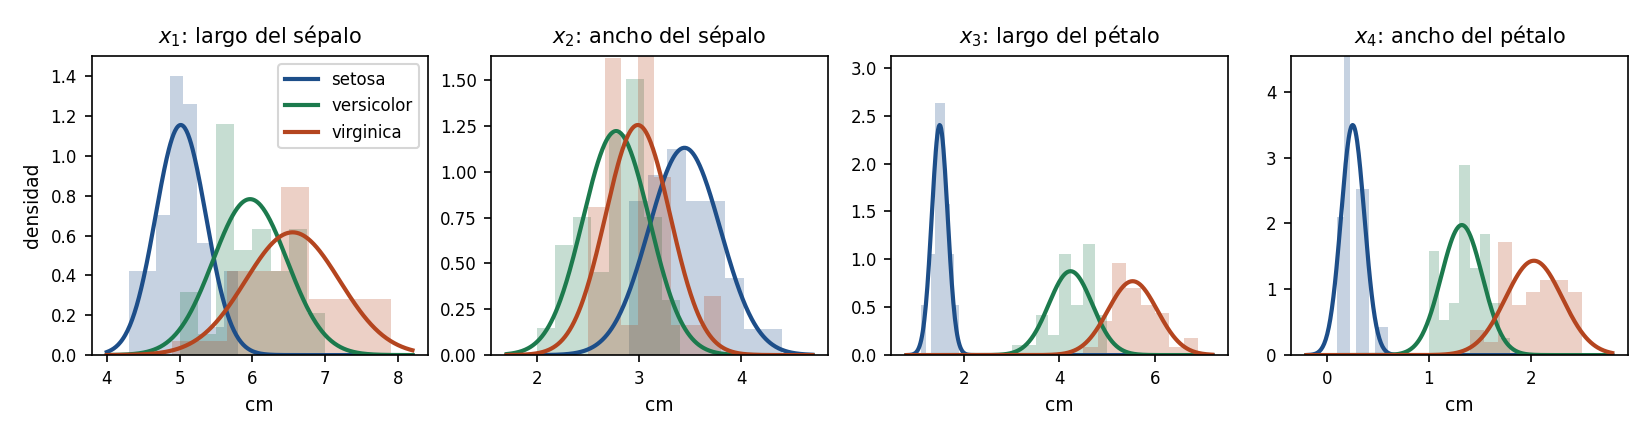
\includegraphics[width=\textwidth]{figures/ej1_campanas.png}
\caption{Lo que aprende el clasificador del ejercicio~\ref{ej:iris}: para cada atributo, la campana de Gauss de cada variedad, sobre el histograma de sus flores de entrenamiento.}
\label{fig:campanas}
\end{figure}

\begin{exercise}[breakable]\label{ej:iris}
Complete las funciones de \texttt{naive\_bayes/gaussiano.py} y ejecute \texttt{1\_iris\_main.py} después de cada apartado.
\begin{enumerate}
    \item[a)] \textbf{Entrenar} (\texttt{entrenar\_naive\_bayes}). Para cada variedad, $P(c)$ y la media y la desviación típica de cada atributo, solo con las flores de esa variedad. Prográmelo: el programa entrena con las 114 flores de entrenamiento, escribe la media y la desviación típica de cada atributo en cada variedad y dibuja sus campanas (figura~\ref{fig:campanas}). En el largo del pétalo, las medias deben ser 1,4921, 4,2316 y 5,5316~cm, y las desviaciones típicas, 0,1660, 0,4554 y 0,5171~cm. Mire la figura: ¿qué atributo separa mejor las tres variedades? ¿Entre qué dos variedades espera que se equivoque el clasificador?
    \item[b)] \textbf{Clasificar una flor.} La función \texttt{log\_densidad\_gaussiana} calcula $\log P(x_i \mid c)$ de un valor $x_i$, con la media y la desviación típica de su atributo en la clase $c$, y la función \texttt{calcular\_puntuaciones}, la puntuación de cada clase, $\log P(c) + \sum_i \log P(x_i \mid c)$, con un bucle por clase y, dentro, otro por atributo. Prográmelas: el programa clasifica la primera flor de test, $x = (5{,}0;\ 3{,}6;\ 1{,}4;\ 0{,}2)$, y escribe, para cada variedad, $\log P(c)$ y el logaritmo de cada atributo, y después la puntuación. La puntuación debe ser 0,939 para \textit{setosa}, y $-40{,}420$ y $-59{,}571$ para \textit{versicolor} y \textit{virginica}. Calcule a mano $\log P(x_3 = 1{,}4 \mid \textit{setosa})$, con la media y la desviación típica del apartado a), y compruebe que sale 0,723. ¿Cómo puede ser positivo el logaritmo de una probabilidad?
    \item[c)] \textbf{Las flores de test.} \texttt{predecir\_naive\_bayes}, ya programada, devuelve la clase de mayor puntuación. El programa clasifica con ella las 36 flores de test y escribe la tasa de acierto, que debe ser del 94,4\,\% (del 96,5\,\% en las de entrenamiento), y la \textbf{matriz de confusión}: cuántas flores de cada variedad (filas) se han clasificado como cada variedad (columnas). ¿Qué variedades se confunden? ¿Es lo que esperaba en a)? ¿Por qué se mide el acierto con flores que no se han usado para entrenar? Por último, el programa entrena \texttt{GaussianNB} de \texttt{scikit-learn} con las mismas flores y comprueba que hace las mismas predicciones que sus funciones.
\end{enumerate}
\end{exercise}


\section{La bolsa de palabras}
La aplicación más famosa de Naïve Bayes es el filtro de spam: fue el primer método que funcionó de verdad, y durante años lo llevaron todos los gestores de correo. Usaremos la \textbf{SMS Spam Collection} (Almeida y otros, 2011): 5.574 SMS reales, en inglés, etiquetados como \texttt{ham} (legítimo) o \texttt{spam}. Solo 747 son spam, el 13,4\,\%. Se reparten, como las flores, en 4.180 de entrenamiento y 1.394 de test, con la misma proporción de spam en los dos conjuntos.

Un clasificador no sabe leer: necesita números. La \textbf{bolsa de palabras} (\textit{bag of words}) construye un \textbf{vocabulario} con todas las palabras distintas de los mensajes de entrenamiento, en orden alfabético y numeradas desde el 0, y convierte cada mensaje en un vector con el número de veces que aparece en él cada palabra del vocabulario: la palabra de índice $i$ es la columna $i$. Se pierde el orden de las palabras (de ahí lo de «bolsa»), pero se conserva cuáles aparecen y cuántas veces. Para partir un mensaje en palabras, \texttt{tokenizar}, ya programada, lo pasa a minúsculas, quita los signos de puntuación y descarta las palabras de una sola letra. Una palabra que no está en el vocabulario se \textbf{ignora}: es lo que pasa cuando un mensaje nuevo trae una palabra que no se vio al entrenar.

\begin{exercise}[breakable]\label{ej:bolsa}
En \texttt{naive\_bayes/bolsa\_de\_palabras.py} hay que completar dos funciones. La primera, \texttt{construir\_vocabulario}, construye el vocabulario: un diccionario que da el índice de cada palabra. La segunda, \texttt{vectorizar}, convierte una lista de mensajes en su matriz de conteos, con un mensaje por fila. Después, ejecute \texttt{2\_bolsa\_de\_palabras\_main.py}.
\begin{enumerate}
    \item[a)] \textbf{Tres mensajes.} Antes de programar, escriba a mano el vocabulario y la matriz de conteos de estos tres mensajes de entrenamiento: \texttt{'Win a FREE prize now'}, \texttt{'Call me now'} y \texttt{'I win, you win'}, y el vector correspondiente al mensaje de test \texttt{'Call now to win a prize'} a partir del vocabulario. Prográmelo y compare: el programa construye el vocabulario con los tres mensajes de entrenamiento, escribe su matriz de conteos y convierte en un vector el cuarto mensaje. ¿Por qué hay solo 7 palabras en el vocabulario? ¿Qué pasa con \texttt{to}?
    \item[b)] \textbf{Los SMS.} El programa hace lo mismo con los 4.180 SMS de entrenamiento: el vocabulario tiene 7.498 palabras, y la matriz, de $4.180 \times 7.498$, tiene un 99,82\,\% de ceros. ¿Por qué casi todo son ceros? 
\end{enumerate}
\end{exercise}


\section{Naïve Bayes multinomial: un filtro de spam}
Con la bolsa de palabras, los atributos de un mensaje son los conteos $x_i$ de las palabras $w_i$ del vocabulario $V$, y la probabilidad de la palabra $w$ en un mensaje de la clase $c$ se estima contando:
\[
P(w \mid c) = \frac{N(w, c) + \alpha}{N(c) + \alpha\,|V|}
\]
$N(w, c)$ es el número de veces que aparece la palabra $w$ en todos los mensajes de entrenamiento de la clase $c$, y $N(c)$, el total de palabras de esos mensajes. $\alpha$ es el \textbf{suavizado de Laplace}: se suma $\alpha$ a todos los conteos, como si cada palabra se hubiera visto $\alpha$ veces más en cada clase (en el filtro, $\alpha = 1$), y el $\alpha\,|V|$ del denominador hace que las probabilidades sigan sumando 1. Una palabra que sale varias veces en un mensaje cuenta varias veces, así que la regla de decisión, con la puntuación de cada clase entre corchetes, queda:
\[
c^* = \arg\max_c \; \Big[ \log P(c) + \sum_{i=1}^{|V|} x_i \log P(w_i \mid c) \Big]
\]

\begin{exercise}[breakable]\label{ej:spam}
Complete las funciones de \texttt{naive\_bayes/multinomial.py} y ejecute \texttt{3\_spam\_main.py} después de cada apartado. El programa usa su bolsa de palabras del ejercicio~\ref{ej:bolsa} para convertir los SMS en números.
\begin{enumerate}
    \item[a)] \textbf{Entrenar} (\texttt{entrenar\_naive\_bayes\_multinomial}). Para cada clase, $\log P(c)$ y $\log P(w \mid c)$ de todas las palabras del vocabulario. Prográmelo: el programa entrena el filtro con los 4.180 SMS de entrenamiento y escribe $P(c)$, que debe ser 0,866 para \texttt{ham} y 0,134 para \texttt{spam}, y lo que ha aprendido de la palabra \texttt{prize}: sale 77 veces en el spam y ninguna en los mensajes legítimos, y $\log P(\textit{prize} \mid c)$ vale $-10{,}9097$ en \texttt{ham} y $-5{,}5732$ en \texttt{spam}. Después lo entrena con $\alpha = 0{,}5$ y comprueba que las probabilidades son las de \texttt{MultinomialNB} de \texttt{scikit-learn}. Sin el suavizado ($\alpha = 0$), ¿cuánto valdría $P(\textit{prize} \mid \texttt{ham})$? ¿Qué le pasaría entonces a un mensaje legítimo que dijera \texttt{prize}? Tenga en cuenta que 6.626 de las 7.498 palabras del vocabulario no salen nunca en una de las dos clases.
    \item[b)] \textbf{Clasificar.} La función \texttt{calcular\_puntuaciones\_multinomial} calcula, para un mensaje, la puntuación de cada clase: el corchete de la regla de decisión. Prográmela con dos bucles, uno que recorre las clases y, dentro, otro que recorre las palabras del vocabulario. La función \texttt{predecir\_naive\_bayes\_multinomial}, ya programada, devuelve la clase de mayor puntuación. El programa escribe la puntuación del primer SMS de test, que debe ser $-120{,}816$ para \texttt{ham} y $-143{,}235$ para \texttt{spam}, y clasifica los 1.394 SMS de test. El filtro debe acertar el 97,9\,\%, con 8 mensajes legítimos marcados como spam (\textbf{falsos positivos}) y 21 spam que se cuelan (\textbf{falsos negativos}). Escribe también la \textbf{precisión} del spam (de los mensajes marcados como spam, cuántos lo son: el 95,4\,\%) y su \textbf{accuracy} (de los spam que hay, cuántos se marcan: el 88,8\,\%): compruebe las dos cuentas con la matriz de confusión. Por último, el programa entrena \texttt{MultinomialNB} de \texttt{scikit-learn} con la misma matriz y comprueba que hace las mismas predicciones.
    \item[c)] \textbf{¿En qué se fija el filtro?} El programa escribe las 10 palabras más \textbf{frecuentes} de cada clase, las de mayor $P(w \mid c)$, y las 10 más \textbf{indicativas} de cada una, las de mayor diferencia entre $\log P(w \mid \texttt{spam})$ y $\log P(w \mid \texttt{ham})$, en un sentido y en el otro. Las indicativas del spam deben empezar por \texttt{claim}, \texttt{prize} y \texttt{150p}. ¿Por qué las palabras más frecuentes casi no sirven para distinguir el spam?
    % \item[d)] \textbf{Engañe al filtro.} \texttt{python filtro.py} entrena el filtro y clasifica los mensajes que usted escriba. De cada uno dice si es spam, con $P(\texttt{spam} \mid \text{mensaje})$, el peso de cada palabra, $\log P(w \mid \texttt{spam}) - \log P(w \mid \texttt{ham})$, y las palabras que no conoce, que no cuentan. Escriba un mensaje que sea claramente spam pero que el filtro dé por legítimo, y explique por qué lo ha conseguido.
\end{enumerate}
\end{exercise}


\begin{idea}[title=\textbf{Para terminar}]
\centering
\small
\begin{tabular}{lcc}
\toprule
 & Gaussiano (iris) & Multinomial (spam) \\
\midrule
Atributos & 4 medidas en cm & 7.498 conteos de palabras \\
$P(x_i \mid c)$ & una campana de Gauss & la frecuencia de la palabra, suavizada \\
Entrenar es\dots & calcular medias y desviaciones & contar palabras \\
Todo lo que sabe & $3 + 24$ números & $2 + 2 \times 7.498$ números \\
Acierto en el test & 94,4\,\% & 97,9\,\% \\
\bottomrule
\end{tabular}

\raggedright
\medskip
Entrenar un Naïve Bayes es contar, con una sola pasada por los datos. La hipótesis ingenua es casi siempre falsa, pero para decidir basta con que la clase correcta salga la mayor. Y el modelo se puede interpretar: se le puede preguntar por qué ha decidido lo que ha decidido, algo que se pierde en modelos más potentes, como las redes neuronales.
\end{idea}

\subsection*{Bibliografía}
\begin{itemize}\small\setlength{\itemsep}{1pt}
    \item Russell, S. y Norvig, P. \textit{Artificial Intelligence: A Modern Approach}, 4.ª ed.: la regla de Bayes y los modelos Naïve Bayes, en el capítulo \textit{Quantifying Uncertainty}, y cómo se aprenden, en \textit{Learning Probabilistic Models}.
    \item Fisher, R. A. \textit{The use of multiple measurements in taxonomic problems}. Annals of Eugenics 7 (1936): las flores iris.
    \item Sahami, M., Dumais, S., Heckerman, D. y Horvitz, E. \textit{A Bayesian approach to filtering junk e-mail}. AAAI Workshop on Learning for Text Categorization (1998): el filtro de spam con Naïve Bayes.
    \item Almeida, T. A., Gómez Hidalgo, J. M. y Yamakami, A. \textit{Contributions to the study of SMS spam filtering: new collection and results}. ACM DocEng (2011): los SMS.
\end{itemize}

\end{document}
